\chapter{State of the Art v oblasti HPC-as-a-Service}
Superpočítače a jejich výkon byl v minulosti vyhrazen pouze pro oblast výzkumu a vývoje. HPC bylo k dispozici vládním, lékařským, výzkumným organizacím a inovativním filmařům. K majoritním případům užití superpočítačů v této době patřily simulace jaderných testů, mapování lidského genomu nebo oživování dinosaurů ve filmech.

V současné době však dochází k masivnímu vzestupu datově náročných technologií. Typickým příkladem může být problematika umělé inteligence nebo problémy vyžadující masivní paralelismus\footnote{Masivní paralelismus je technika využívající velkého počtu procesorů či samotných počítačů k paralelnímu zpracování úloh.}. Tento fakt nutí širší okruh organizací zkoumat problematiku vysoce výkonného počítání. Ne každá společnost však má čas, peníze a odborné znalosti potřebné k jejich nasazení.

Z toho důvodu mohou tyto společnosti namísto náročného sestavování a správ superpočítačových clusterů využít již hotová řešení HPC jako služby (HPC-as-a-Service/HaaS). Díky HPC poskytovanému jako služba mohou organizace v některých případech spolupracovat s dodavatelem na konfiguraci infrastruktury, kterou potřebují pro své konkrétní výpočetní potřeby. Namísto nákupu nebo pronájmu hardwaru či softwaru si je však předplatí prostřednictvím modelu spotřeby „pay-as-you-go“.\cite{Rand20201203}

\section{Výhody HPC-as-a-Service}
HPC poskytované jako služba má výhody oproti hostování vlastní HPC infrastruktury. První důležitou výhodou může být model spotřeby „pay-as-you-go“, který byl již zmiňován výše. Zákazník tak platí jen za zdroje, které skutečně využil. Vlastní řešení, konstrukce a následná správa vysoce výkonných výpočetních clusterů je velmi náročná na zdroje.

Společnosti či organizace poskytující HPC-as-a-Service mají tendenci rychleji integrovat novější technologie. Tyto technologie jsou pak přístupné uživatelům využívající jejich služeb. Někteří poskytovatelé HaaS umožňují jejich zákazníkům provádění aktualizací či škálování\footnote{Škálování je pojem vyjadřující navyšování kapacit.} výpočetních kapacit na vyžádání. \cite{Wiggers20220120}

\section{Případy užití}
V dnešní době se poskytovatelé HPC-as-a-Service snaží co nejvíce přizpůsobit požadavkům jejich zákazníků. HaaS využívají společnosti, které pro řešení jejich problémů většinou vyžadují vysoký výkonného paralelní zpracování dat. Poměrně velký segment zákazníků tvoří oblast Automotive\footnote{Segment automobilového průmyslu.}, ti využívají HPC například ke zkrácení času simulací proudění tekutin či plynů. Při využití výpočetních clusterů nejen oboru Automotive dochází přesnějším a rychleji dosaženým výsledkům při vývoji. Dalším oborem, ve kterém je HPC hojně využíváno je obor lékařství, vývoj léčiv je díky masivnímu paralelnímu zpracovaní efektivnější a rychlejší, dochází pak i k minimalizaci vzniku chyb.

HPC je využíváno v mnoha dalších oborech či odvětvích, patří tam i obor výzkumu a vývoje. HPC umožňuje analyzovat rozsáhlé datové soubory v poměrně krátkém čase a sdílet výsledky se spolupracovníky. Dále je HPC využíváno třeba ke 3D modelování a renderování scén, toho využívají grafická,herní a filmová studia.

Obrázek \ref{fig:haas} ilustruje využití HPC-as-a-Service / HaaS.

\begin{figure}[!h]
	\centering
	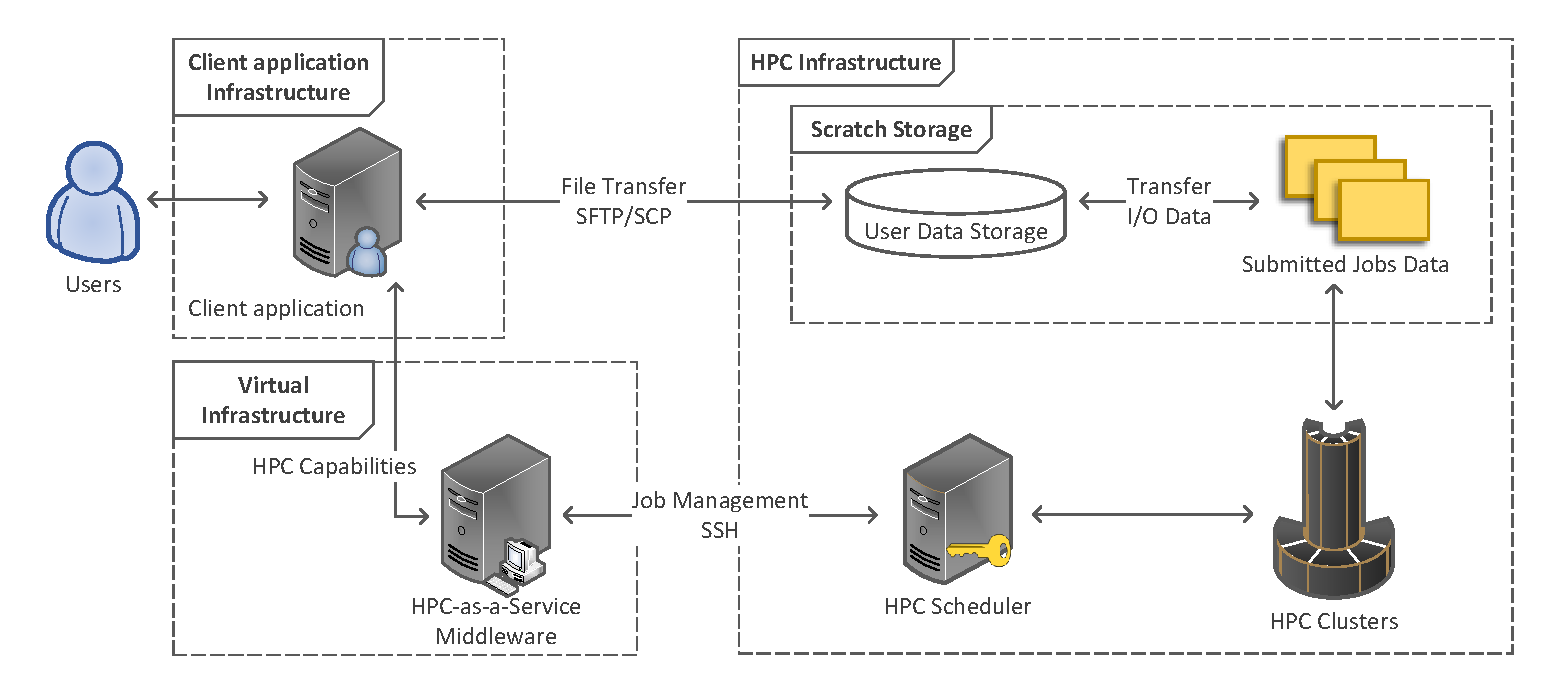
\includegraphics[width=1\textwidth]{Figures/haas.pdf}
	\caption{HPC-as-a-Service / HaaS \cite{uG7wIvjQiIli6kO9}}
	\label{fig:haas}
\end{figure}